\documentclass[12pt]{article}
\usepackage{sbc-template} 
\usepackage{graphicx,url}
\usepackage{url}
\usepackage[brazil]{babel} 
\usepackage[utf8]{inputenc} 
\usepackage[T1]{fontenc}
\usepackage[normalem]{ulem}
\usepackage[hidelinks]{hyperref}

\usepackage[square,authoryear]{natbib}
\usepackage{amssymb} 
\usepackage{mathalfa} 
\usepackage{algorithm} 
\usepackage{algpseudocode} 
\usepackage[table]{xcolor}
\usepackage{array}
\usepackage{titlesec}
\usepackage{mdframed}
\usepackage{listings}

\usepackage{amsmath} 
\usepackage{booktabs}

\urlstyle{same}

\newcolumntype{L}[1]{>{\raggedright\let\newline\\\arraybackslash\hspace{0pt}}m{#1}}
\newcolumntype{C}[1]{>{\centering\let\newline\\\arraybackslash\hspace{0pt}}m{#1}}
\newcolumntype{R}[1]{>{\raggedleft\let\newline\\\arraybackslash\hspace{0pt}}m{#1}}

\newcommand\Tstrut{\rule{0pt}{2.6ex}} 
\newcommand\Bstrut{\rule[-0.9ex]{0pt}{0pt}} 
\newcommand{\scell}[2][c]{\begin{tabular}[#1]{@{}c@{}}#2\end{tabular}}

\usepackage[nolist,nohyperlinks]{acronym}

\title{Real Time Detection of Pump-and-Dump Schemes in Cryptocurrency Markets}

\author{Matheus Moura\inst{1}}


\address{Centro Federal de Educação Tecnológica Celso Suckow da Fonseca - CEFET/RJ
	\email{matheus.moura@aluno.cefet-rj.br}
}



\begin{document} 
	
	\maketitle
	
	\begin{resumo} 
		Este roteiro traz as principais informações para a elaboração de trabalhos científicos. o trabalho deve ser escrito de modo a se mostrar interessante e importante. Para tanto, a forma de escrevê-lo, principalmente no resumo e  introdução, é fundamental. É o momento no qual o autor deve ``vender o trabalho''. 
		
		Em textos científicos, as frases devem ser curtas, para não gerar ambiguidade. Pode-se dizer que um parágrafo é constituído por pelo menos três frases. Adicionalmente, pode-se dizer que cada parágrafo tem uma única ideia central, \emph{i.e.}, uma sentença  que sumariza o parágrafo. 
		
		O texto de um trabalho todo precisa estar encadeado \citep{zobel_writing_2015}. O encadeamento dos parágrafos é feito a partir do encadeamento de suas ideias centrais. Desta forma, a ideia central de cada parágrafo leva a ideia central do próximo e assim por diante. 
		
		Em linhas gerais, qualquer parágrafo do trabalho que não apresente citação é considerado criação dos autores. A utilização de textos transcritos de alguma fonte sem a devida referência a esta fonte e seus autores pode configurar a hipótese de plágio. Assim, todas as obras citadas devem ter as referências aos seus autores e devem figurar na lista de referências do trabalho.
	\end{resumo}
	
	\section{Introdução}
	\label{sec_introducao}

	The adoption of cryptocurrencies has experienced significant growth over the past decade, leading to a substantial expansion of the market both within traditional financial sectors and in public perception.
	This trend is exemplified by notable milestones, such as the approval of the first Bitcoin futures Exchange-traded fund (ETF) by the U.S. Securities and Exchange Commission (SEC) in 2021 \citep{wursthorn2021} and the trading commencement of spot ETFs on American stock exchanges in early 2024 \citep{schmitt2024}.
	The surge in public interest can be attributed to the exponential growth observed in the cryptocurrency market during late 2017 and early 2018, which captured widespread attention from mainstream media, attention that recurs with each subsequent occurrence of high bullish market trends \citep{steinmetz2021}.
	Consequently, there is a pressing need for comprehensive studies to assess the risks associated with this fairly new asset class.

	The vast majority of cryptocurrencies operate without reliance on any central authority and offer a degree of anonymity.
	These features facilitate their utilization in illicit activities, including but not limited to money laundering, drug trafficking, and hacking \citep{Kethineni2019}.
	Among the various fraudulent practices associated with cryptocurrencies, one prominent scheme is the pump-and-dump (P\&D) scheme, characterized by the artificial inflation of an asset's price followed by the sale of the acquired assets at a higher price \citep{li2021}.

	Organizers of pump-and-dumps leverage on social media platforms that offer some level of anonimity, such as Telegram and Discord.
	Where they establish a public group or channel and recruit as many members as possible for what are colloquially termed "pump groups".
	Within these groups only scheme organizers are allowed publishing messages and once a critical mass of members is attained, typically exceeding 1,000, operations commence \citep{xu2019}.

	The typical modus operandi of these groups starts with the dissemination of precise details, including the exact date, time, and exchange where the pump-and-dump operation will occur, allowing members adequate time to prepare their funds.
	At the pre-arranged time, the group administrators announce the targeted cryptocurrency and encourage members to acquire and retain it to artificially inflate its price.
	Throughout the pumping phase, participants promote the targeted coin on social media platforms to attract external attention.
	However, in a few minutes the price peak is reached and the participants begin panic-selling at the first sign of decline, leading to a rapid return of the coin's price to its pre-pump level \citep{xu2019}.

	Therefore, the detection of pump-and-dump holds significance in mitigating victimization and aiding market participants in identifying and addressing this kind of market manipulation.
	Pump-and-dump schemes manifest as anomalies within the time series data of the targeted cryptocurrency's price.
	This study investigates model deviation detection methods, a widely employed strategy for anomaly identification.
	This approach involves identifying events where there is a discrepancy between the observed behavior of the time series and the anticipated behavior as forecasted by a model \citep{ogasawara2024}.
	In contrast, our results are compared with that of \citet{lamorgia2020}, who employed a classification method for anomaly detection.
	They extracted a set of features from the time series data of the pumped cryptocurrency and utilized machine learning algorithms for classification.

	

	\# Which approach was used in this work and how well it performed. (contributions)

	\# Work structure.
	
	A estrutura do trabalho é comumente apresentada no último parágrafo da introdução. Cabe salientar que um trabalho não é um romance, isto é, não devem aparecer elementos surpresas ao longo do texto. O texto é elaborado e apresentado de modo bem organizado e planejado. 
	
	\section{Theoretical Foundation}
	\label{sec_fund_teorica}

	The pump-and-dump scheme has a long history in the stock market \citep{lamorgia2020}.
	The subsequent subsection, "Pump-and-Dump Definition" (see Subsection \ref{subsec_pump_def}) examines its operation within traditional stock markets.
	Following this examination, the subsection "Pump-and-Dump in Cryptocurrency Markets" (see Subsection \ref{subsec_pump_in_crypto}) explains why cryptocurrency markets are susceptible to the scheme and how the scheme has been adapted.

	\subsection{Pump-and-Dump on Traditional Stock Market}
	\label{subsec_pump_def}

	The pump-and-dump scheme operates on a straightforward premise.
	Initially, the perpetrators identify a publicly traded security, typically of small size and with low trading volumes, as their target.
	Subsequently, they accumulate significant quantities of this security.
	Following acquisition, they start tounting the security, disseminating false and misleading information aimed at artificially inflating its price \citep{kramer2005}.

	Since the rise of the internet, anyone has been able to reach mass audiences, which created this new age of decentralized information.
	Concurrently, internet has facilitated the propagation of fraudulent activities reliant on information dissemination, which can now spread through various channels such as social media platforms, investment research websites, investment newsletters, online advertisements, and others.
	An early example of the pump-and-dump scheme's adaptation to the stock market using the internet occurred with the emergence of the website Fast-Trades.com in 1999.

	Fast-Trades operated as a stock selection website, providing recommendations to its subscribers while employing a six-month trial period to attract new users.
	The modus operandi was straightforward: the website owner and his friends initiated stock purchases prior to their disclosure as selections, concurrently placing sell limit orders\footnote{In this kind of order you set the lowest amount you would be willing to accept for each share you sell.}.
	Through this strategy, the perpetrators were able to profit several times the purchase price.
	For instance, their inaugural selection, Apache Medical Systems, saw its price surge to 600\% above the rate at which the site owner had purchased \citep{kramer2005}.

	During that time, the internet was a novel frontier, affording Fast-Trades.com perpetrators the opportunity to orchestrate the pump-and-dump scheme with minimal expertise in the stock market.
	Nevertheless, despite the internet's enabling role, it did not guarantee anonymity in their trades, as the stock market operates under centralized authorities with monitoring capabilities, which enabled regulators to uncover the scheme \citep{kramer2005}.
	Thus, the online fraudsters found themselves navigating a landscape where they possessed a potent means of reaching mass audiences, yet were constrained to operating within centralized and regulated markets.
	
	\subsection{Pump-and-Dump on Cryptocurrency Markets}
	\label{subsec_pump_in_crypto}

	This landscape was changed by \citet{nakamoto2008} with the introduction of Bitcoin and subsequent cryptocurrencies.
	Unlike traditional financial systems, the vast majority of cryptocurrencies operate without central authorities to process transactions, instead utilizing the peer-to-peer technology known as blockchain.
	This egalitarian nature of cryptocurrencies has ushered in a new era of decentralized authority, often affording privacy of transactions, dissociative anonymity, and a lack of deterrence \citep{Kethineni2019}.
	The convergence of these characteristics with the capabilities offered by the internet created a breakthrough, enabling online criminal activities such as the pump-and-dump scheme to proliferate with even more freedom.

	Este capítulo pode ter várias subseções, uma para cada diferente tema abordado. Por exemplo, se o objetivo do projeto final for implementar um jogo computacional de competição em ferramentas de redes sociais, pode-se ter uma subseção tratando os jogos computacionais e seus aspectos e posteriormente outra subseção tratando de redes sociais. Esta organização deve ser bem definida, mas o princípio básico do bom encadeamento deve ser preservado.
	
	
	As Figuras, Tabelas e Equações devem ser numeradas e citadas no texto. A Tabela \ref{tab_exemplo} apresenta um exemplo de tabela. A Figura \ref{fig_exemplo} apresenta um exemplo de figura. A Equação \ref{eq_exemplo} apresenta um exemplo de equação. Cada figura, tabela e equação merece um parágrafo de explicação própria.
	
	\begin{table}[!ht]
		\centering
		\caption{Exemplo de tabela}
		\begin{tabular}{L{1.5cm} R{1.5cm}}
			\toprule
			\textbf{x}  & \textbf{y} \\
			\midrule
			-2  & 4 \\
			-1  & 1 \\
			0  & 0 \\
			1  & 1 \\
			2  & 4 \\
			\bottomrule
		\end{tabular}
		\label{tab_exemplo}
	\end{table}
	
\begin{figure}[!ht]
 \centering
 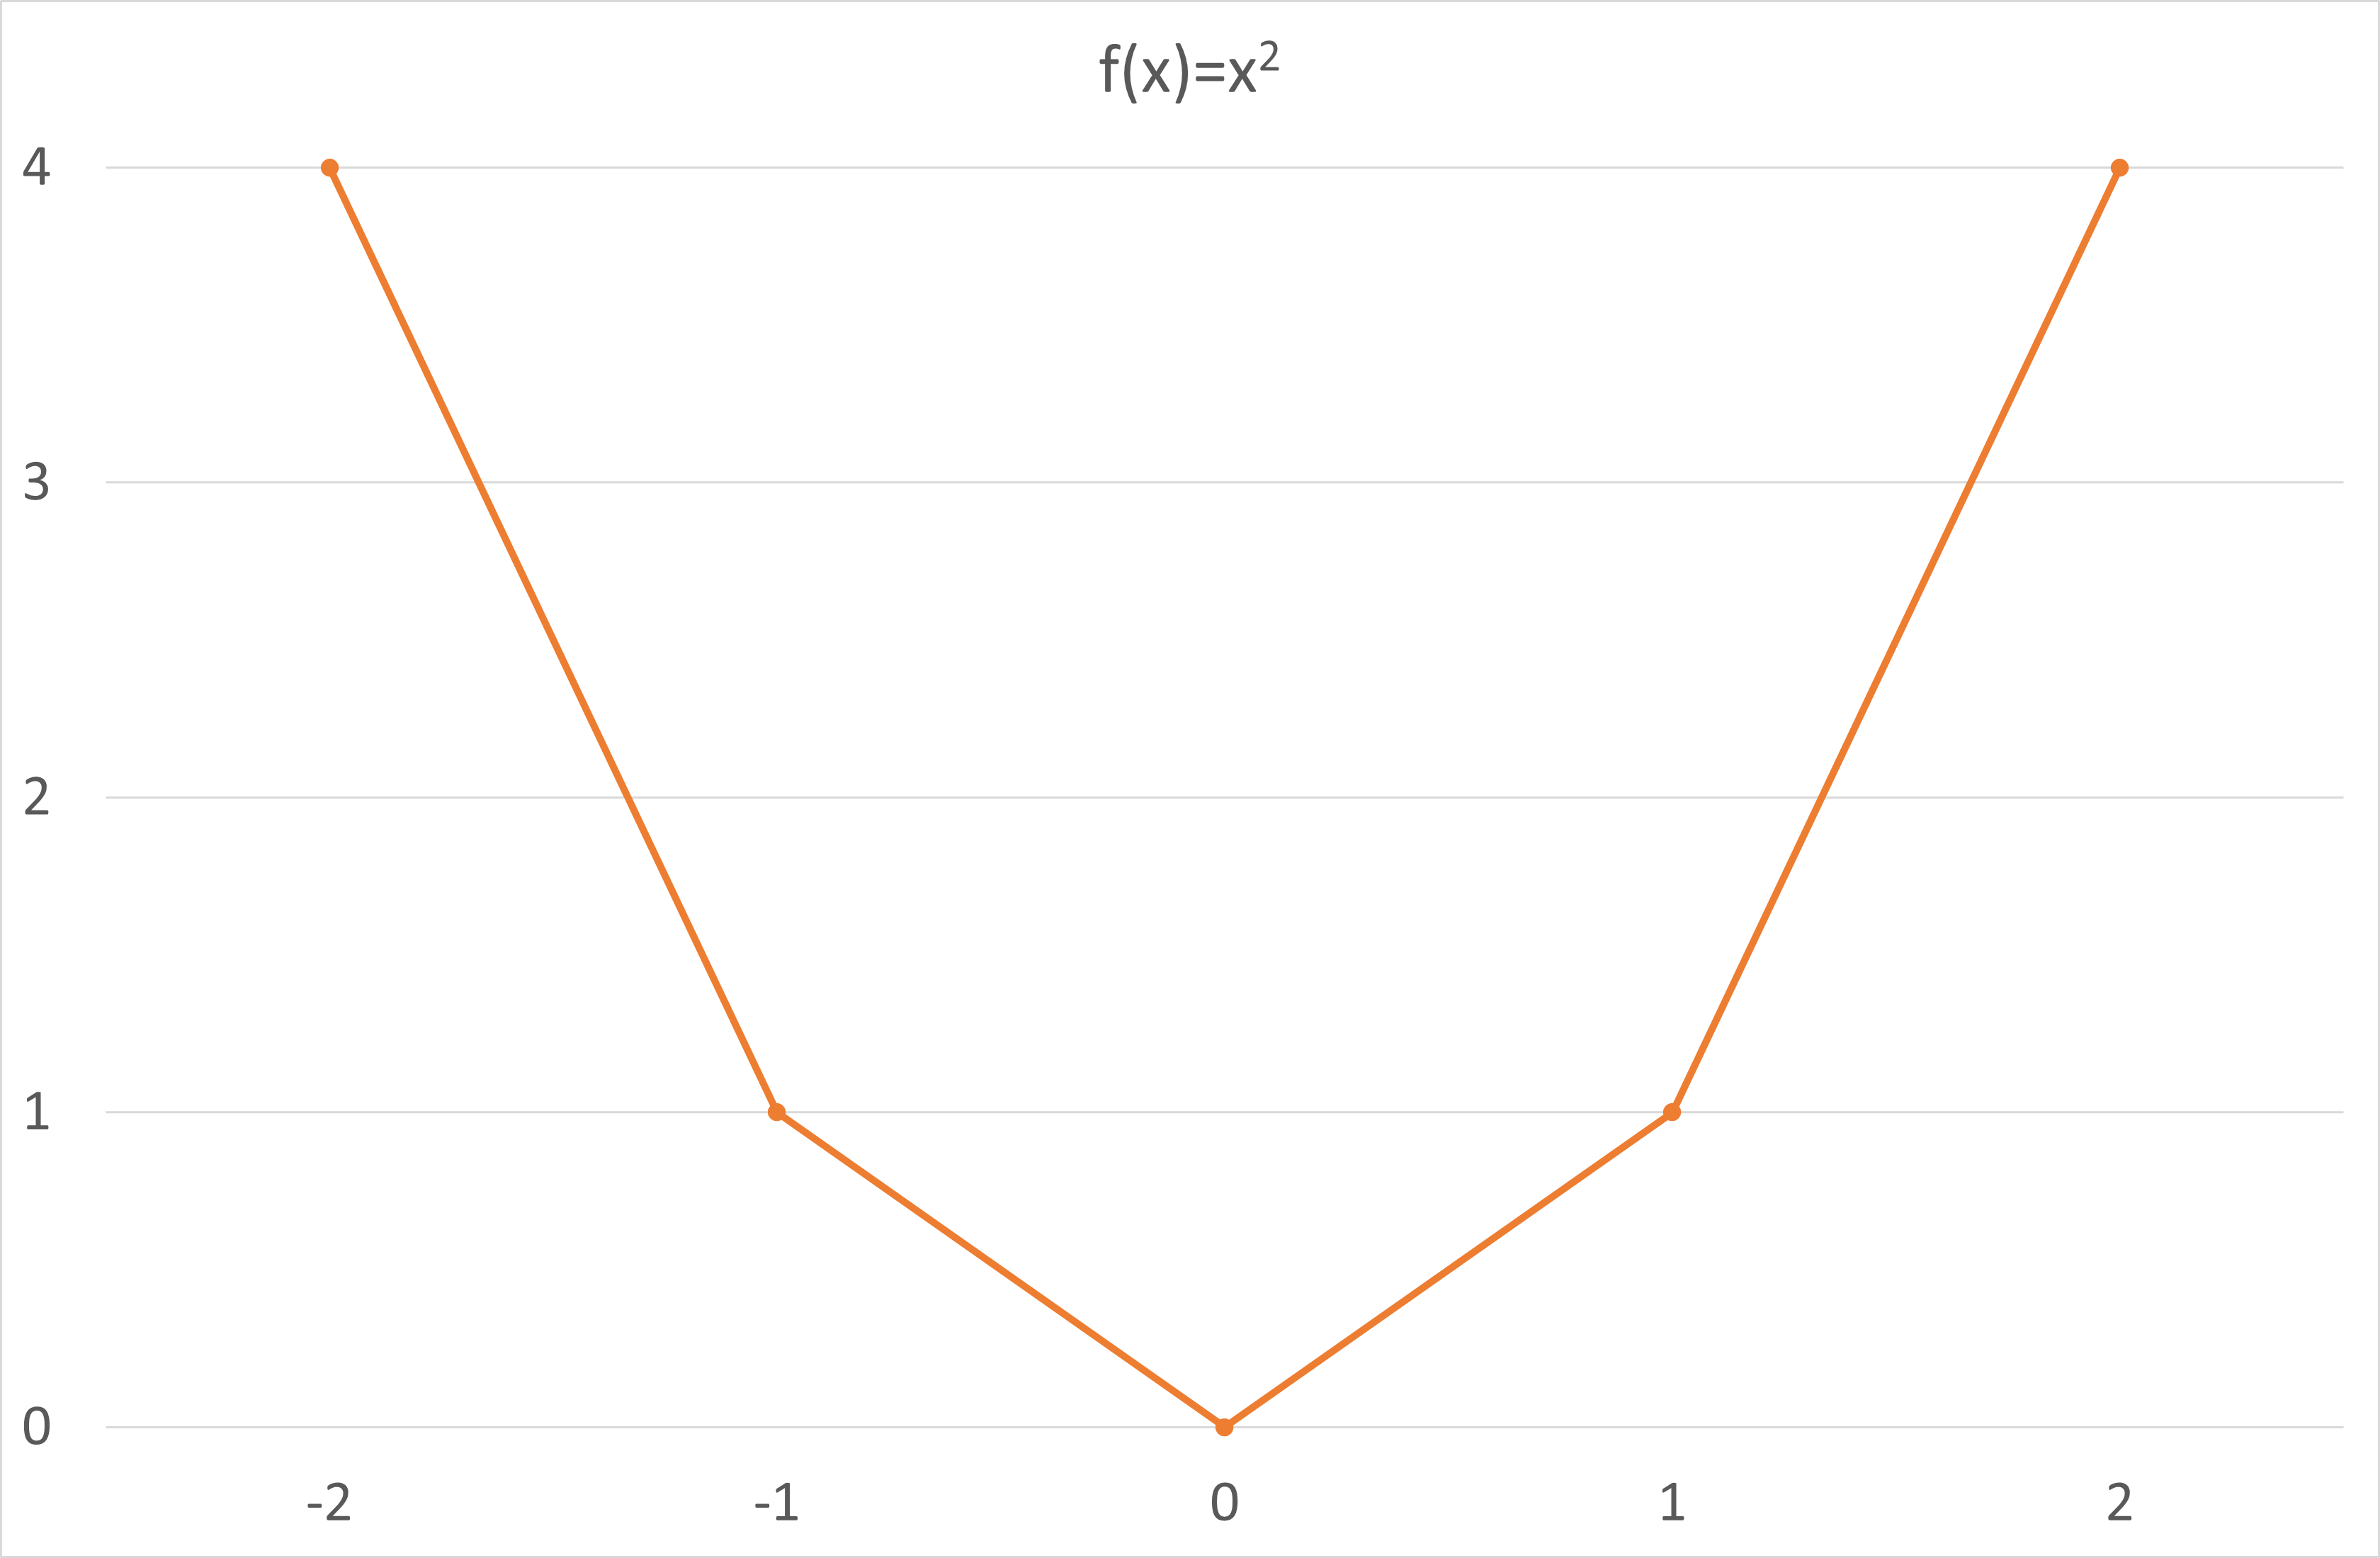
\includegraphics[width=0.6\textwidth]{figures/figura.png}
 \caption{Exemplo de figura}
 \label{fig_exemplo}
\end{figure}	

\begin{equation}
\label{eq_exemplo}
 f(x) = x^2, x \in [-2,2]
\end{equation}


	
	
	\section{Trabalhos relacionados}
	\label{sec_trab_relacionados}
	
	Ao final da fundamentação teórica devem ser apresentados os trabalhos relacionados referentes soluções semelhantes para o problema definido. Os trabalhos relacionados demonstram o estado da arte do tema do trabalho \citep{wazlawick_metodologia_2017}. Descrevemos, resumidamente, os trabalhos e pesquisas já efetuados na área do tema do trabalho, indicando os estudos realizados e os resultados obtidos por seus autores. Esta elaboração deve ser obtida a partir de um mapa sistemático\footnote{Eventualmente esta seção pode ficar depois da avaliação experimental}. 
	
	\section{Método}
	\label{sec_metodo}
	
	O desenvolvimento, juntamente com a avaliação experimental, é um dos núcleos do trabalho. O desenvolvimento compreende a modelagem e a elaboração da solução propriamente dita. Deve ser apresentado de forma ordenada e ampla, com o conteúdo relevante para a apresentação da solução a que o trabalho se propõe. Fica a cargo dos autores estabelecer a estrutura deste capítulo, bem como definir os elementos que devem ser utilizados para elaborar o desenvolvimento da solução. 
	
	A modelagem da solução para a elaboração dos artefatos computacionais define os principais elementos que fazem parte da solução proposta pelo trabalho. Em um sistema de informação, por exemplo, é natural a presença de um diagrama arquitetura, diagrama de caso de uso, um diagrama de classes. Na existência de um processo importante, pode-se recorrer a um diagrama de atividades. Da mesma forma, na existência um procedimento computacional complexo, pode-se fazer valer de especificação de um algoritmo em pseudocódigo, de diagrama de sequência, dentre outros, para explicá-lo. É importante deixar claro que o foco não é volume de elementos de diagramação e diferentes tipos de modelo, mas sim a qualidade da explicação da solução.
	
	A qualidade da explicação está intimamente ligada ao bom encadeamento deste capítulo. Isso significa dizer que se um diagrama for incorporado neste capítulo, cada elemento do diagrama precisa ser explicado. Por exemplo, se for utilizado um diagrama de classe, as principais classes e atributos devem ser apresentados, uma vez que cada uma das classes e cada atributo deve ser explicado no texto.
	
	A elaboração da solução propriamente dita apresenta um detalhamento dos elementos da solução. Pode envolver a especificação da arquitetura da solução, projeto lógico e físico da base de dados, projeto de interface gráfica, linguagem de programação adotada como os seus respectivos \emph{frameworks}. Novamente, o nível de detalhamento dos elementos da solução deve estar condizente com a explicação textual. Não é necessário apresentar todos os elementos da solução. O importante é deixar claro os elementos que valorizem a contribuição do trabalho.
	
	\section{Avaliação experimental}
	\label{sec_aval_exp}
	
	A avaliação experimental compreende uma avaliação quantitativa ou qualitativa do trabalho a partir de critérios estabelecidos para comparação. Como em qualquer experimento, a capacidade de reprodução é fundamental para sua validade. Sendo assim, é importante descrever o processo de experimentação adotados, apresentar os resultados propriamente dito, com uma síntese explicativa dos principais resultados. Finalmente, devem ser apresentadas as ameaças ao estudo, \emph{i.e.}, qualquer coisa que possa tirar ou limitar a validade do experimento conduzido. 
	
	\section{Conclusão}
	\label{sec_conclusao}
	
	A conclusão é a finalização do trabalho e indica as conclusões obtidas com o desenvolvimento do trabalho, sejam elas positivas ou negativas. Nas conclusões, analisa-se o que era desejado (definido na introdução com os objetivos), comparando com o alcançado pelo trabalho, descrevendo como os objetivos foram alcançados e o porquê de algum objetivo não ter sido alcançado. Destacam-se também as contribuições do trabalho, incluindo os benefícios e inovações trazidas pelo trabalho.
	
	Apresentam-se os pontos do trabalho que merecem um maior aprofundamento de estudos. Isso possibilita a criação de novos trabalhos com estudos nesses pontos apresentados, na forma de uma continuidade das pesquisas efetuadas pelo trabalho. Os trabalhos futuros indicam, ainda, uma maturidade de pesquisa do autor do trabalho e esses pontos podem ser trabalhados, posteriormente.
	
	\section*{Agradecimentos}
	Agradecimento as agências de fomento\footnote{Lembre-se de agradecer a CAPES se você tiver usado o Portal de Periódicos}.
	
    \bibliographystyle{apalike}
	\bibliography{references}
	
\end{document}
